\section{Presentación de la arquitectura}

En esta sección presentaremos la arquitectura explicando cómo se brindan las funcionalidades requeridas, mencionando diseños alternativos y algunos aspectos relevantes de la comunicación. Cuando resulte pertinente se comentará cómo se logra cada atributo de calidad a partir de las tácticas utilizadas y la estructura descripta. 


%TODO ver si sirve algo de esto....
Las partes del sistema ser\'an alojadas en diversos lugares f\'isicos. Los usuarios del sistema (votantes y aspirantes a candidatos) podr\'an utilizar al componente \emph{browser usuario externo} desde sus disposivos moviles y computadoras personales. Tambi\'en tendr\'an disponibles terminales en cada sede que estar\'an disponibles en todo momento para utilizar al sistema. Dichas terminales estar\'an conectadas al \emph{Sistema Web} de la sede de manera directa, por lo que ser\'a posible votar y candidatearse cuando la sede se encuentre sin conexi\'on a internet.

Dentro de cada sede se encuentra el componente sede que constar\'a del sistema web, repositorios de datos de usuarios, almacenamiento de votos encriptados y un repositorio de los usuarios que votaron all\'i. 
Los dem\'as componentes de la facultad ser\'an alojadas en la sede donde se encuentre el decanato de la facultad. Por otro lado, el componente \emph{Fiscalizador} ser\'a replicado en varios lugares. Cada facultad tendr\'a uno para fiscalizar las elecciones al finalizarlas. Por otro lado, tambi\'en se encontrar\'a en el componente de agrupaci\'on pol\'itica (es decir, cada agrupaci\'on tendr\'a la posibilidad de fiscalizar las elecciones).

Dentro del rectorado se alojar\'an el servidor de resultados oficiales, administrador de elecciones, administrador de resultados, administrador de datos oficiales de quienes votaron, administrador de actas y una interfaz gr\'afica por la cual se podr\'a configurar los calendarios de elecciones y los reglamentos de las elecciones por medio del \emph{Administrador de elecciones}.

El sistema HardToBreak estamos considerando que es algo externo al sistema y ser\'a alojado por terceros. Tambi\'en consideramos externo el sistema de registros de la facultad.


La sección \ref{explicaciones} contiene explicaciones de varios de los componentes más relevantes y puede resultar útil utilizarla como referencia para ampliar la comprensión de la presente sección.


El uso más habitual que se le dará al sistema será el de votar, por lo que comenzaremos explicando cómo se logra esta funcionalidad con la arquitectura propuesta, enfocándonos principalmente en el diagrama de componentes y conectores.


Para mejorar la seguridad del sistema se eligió utilizar combinaciones de nombre de usuario y contraseña para identificar a los usuarios. Cada usuario tendrá asociado una cuenta, que contendrá además de la información de identificación la preferencia de lenguaje. La creación de cuentas para los usuarios se deberá realizar en una oficina de la sede a la que pertenezca el alumno, donde existirá una terminal segura ejecutando el componente \emph{Administrador de usuarios}\tactica{, apelando, en este caso, a la táctica de seguridad \textit{Limit access} y a \textit{Authenticate User}.} Este componente permitirá crear nuevas cuentas y modificar cuentas existentes. Al momento de creación de la cuenta se solicitará al usuario que ingrese una contraseña. Existían otras alternativas para resolver el problema de administración de cuentas de usuarios que aumentaban la complejidad de la arquitectura y ofrecían menos garantías de seguridad, como generar las contraseñas automáticamente y enviarlas por correo electrónico, o que la creación de cuentas se realice remotamente. En el primer caso la seguridad depende en gran medida del software que cada usuario utilice para ver su correo electrónico, mientras que la segunda opción no ofrece, de la manera que la pensamos, ningún tipo de garantía sobre la identidad de la persona que genera la cuenta.

% TODO agregar diagrama arquitectura completo

\begin{figure}[H]
	\begin{center}
		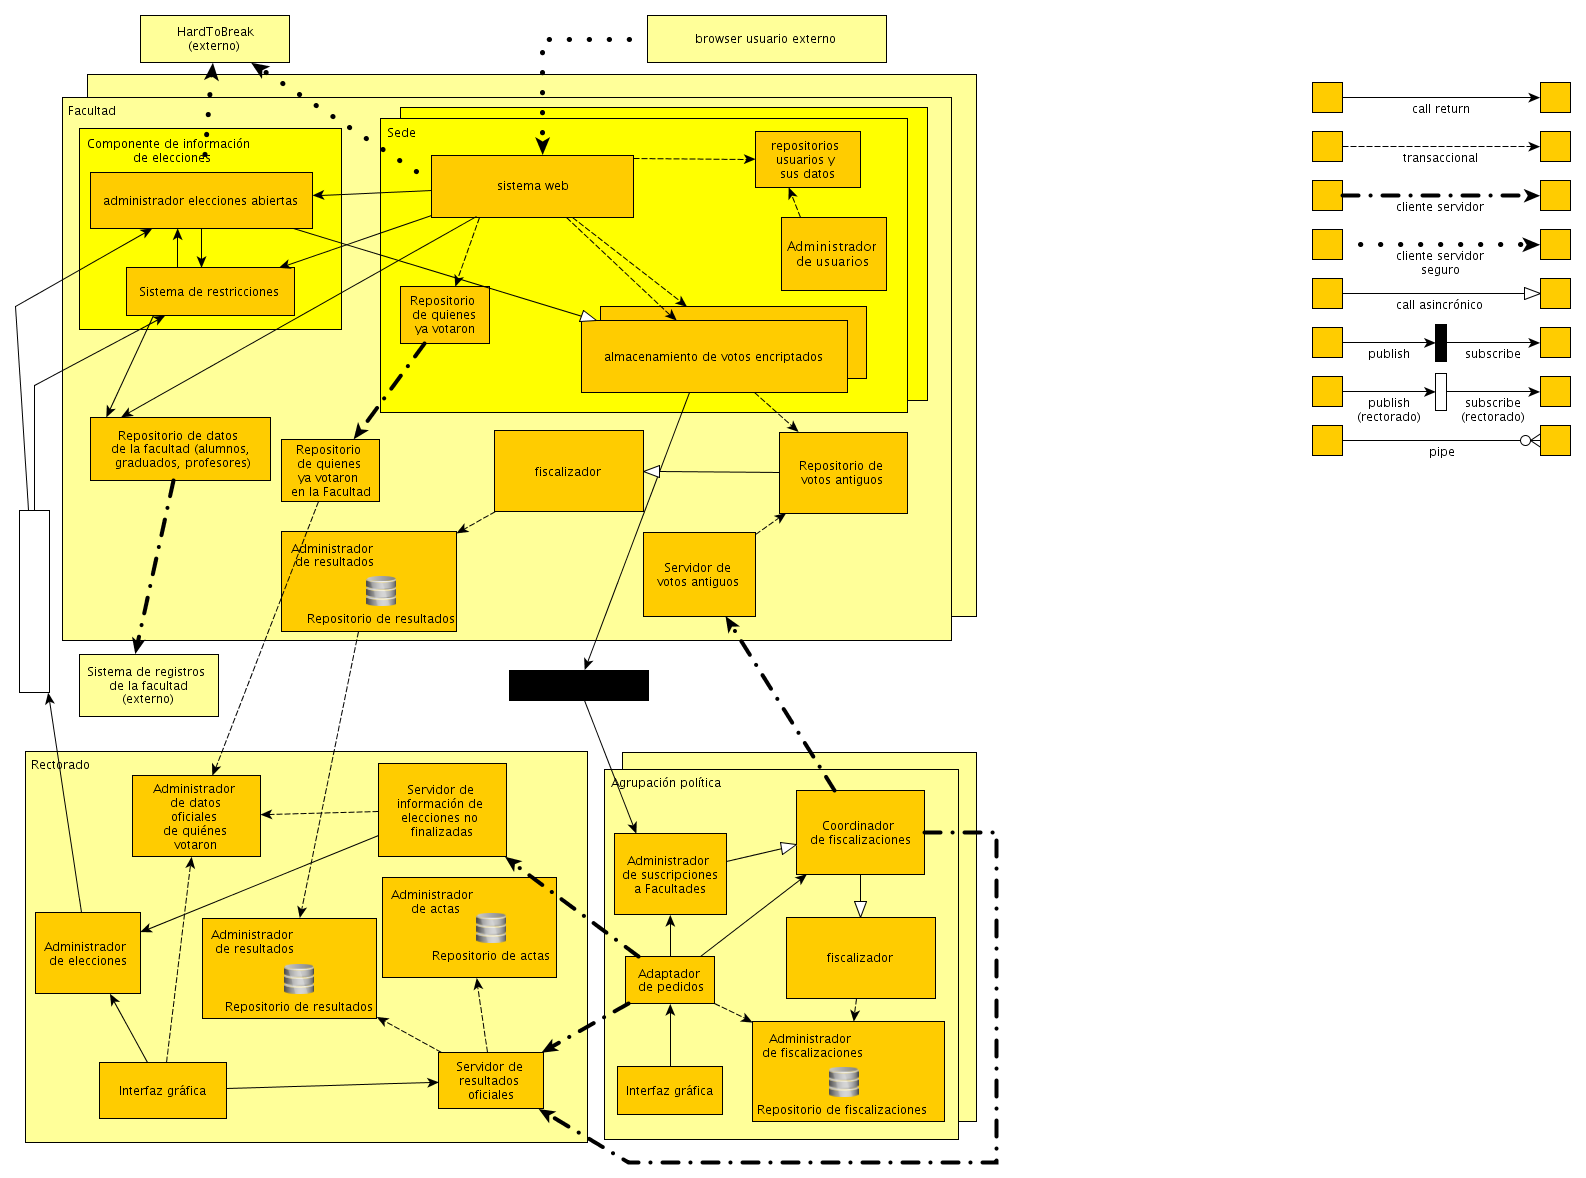
\includegraphics[scale=0.5]{../informe/imagenes/arq1.png}
	\end{center} 
	\caption{Conectores utilizados en la arquitectura}
	\label{fig:tiposConector}
\end{figure}

\begin{figure}[H]
	\begin{center}
		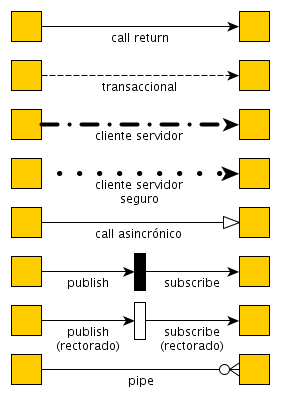
\includegraphics[scale=1]{../informe/imagenes/tipos_conectores.png}
	\end{center} 
	\caption{Componentes y conectores}	
	\label{fig:vistaPrincipal}
\end{figure}

\begin{figure}[H]
	\begin{center}
		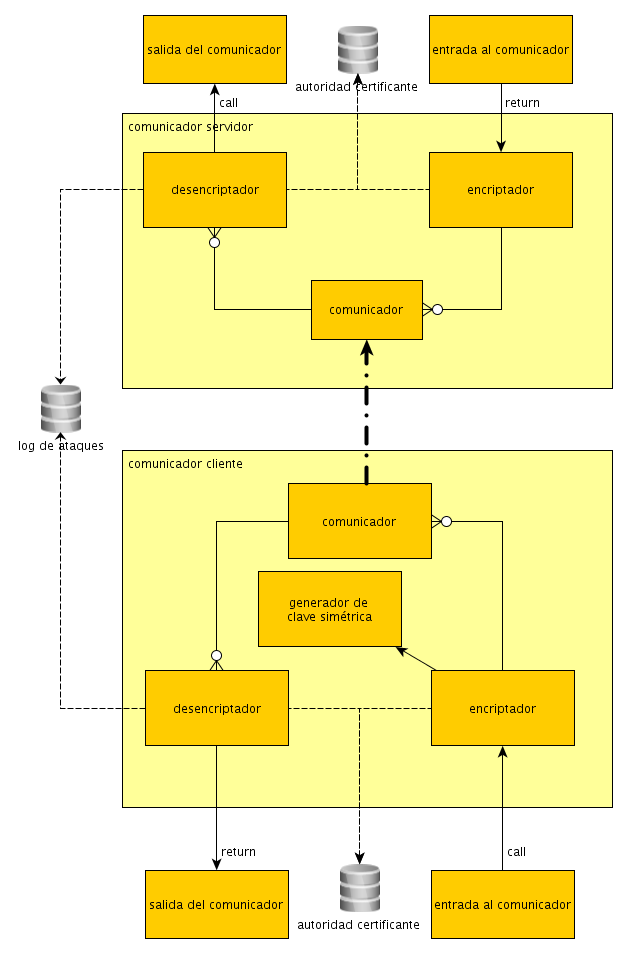
\includegraphics[scale=0.5]{../informe/imagenes/comunicador.png}
	\end{center} 
	\caption{Componentes y conectores del conector cliente servidor seguro}	
	\label{fig:Conector}
\end{figure}

\begin{figure}[H]
	\begin{center}
		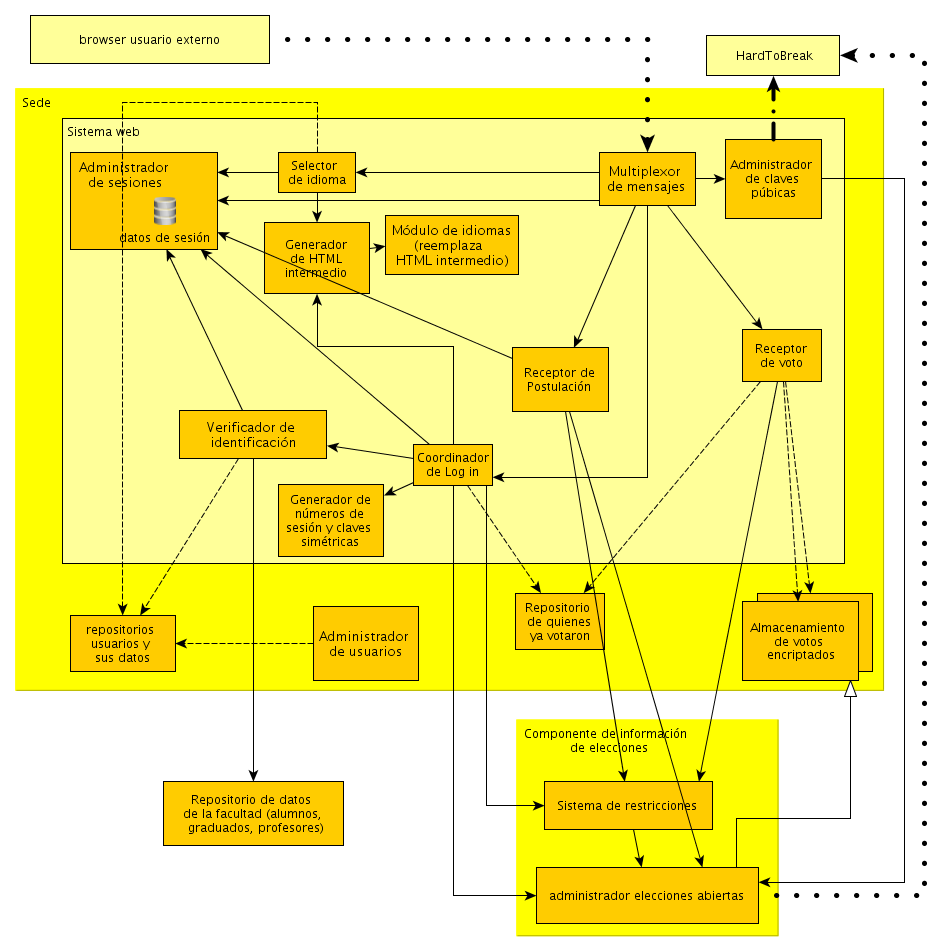
\includegraphics[scale=0.5]{../informe/imagenes/sistema_web.png}
	\end{center} 
	\caption{Componentes y conectores ampliado para el Sistema Web}	
	\label{fig:sistemaWeb}
\end{figure}


El flujo de información durante una votación se describe a continuación. El usuario, a través del componente browser externo, ingresa en un sitio web designado por la Facultad con el fin de realizar la votación.  Este sitio web será exclusivo de la sede a la que un usuario pertenezca, con el objetivo de mejorar la disponibilidad. Para la comunicación entre el browser y la sede de la Facultad utilizaremos una modificación de un conector cliente servidor. La utilización de este conector como parte del estilo arquitectónico del mismo nombre permite mejorar la performance del sistema en general.

El sitio web será generado por el componente sistema web de la sede correspondiente. Existen varios tipos de mensajes posibles entre \emph{browser usuario externo} y \emph{sistema web} que se explicarán en detalle en la sección \ref{mensajes}. 

Cada mensaje está asociado a las diversas acciones que puede querer realizar el usuario. Concretamente, lo único que puede hacer el usuario inicialmente es identificarse con su nombre de usuario y contraseña, tras lo cual se activarán varias opciones adicionales.


Cada recepción de un mensaje genera un nuevo thread de ejecución de algunos de los componentes del sistema web. Los únicos componentes dentro del \emph{sistema web} que procesan serialmente algunos de los pedidos son el  \emph{Administrador de sesiones} y el \emph{Administrador de claves públicas}, ya que ciertos pedidos concurrentes podrían causar conflictos.
Al recibir un mensaje de log in, éste será manejado inicialmente por el \emph{Multiplexor de mensajes}, que lo procesará solicitando al \emph{Coordinador de log in} confirmación de la identidad y una respuesta en formato HTML para responder al usuario. El \emph{Coordinador de log in} se encarga de coordinar la verificación de los datos y la generación de una página con las opciones disponibles para el usuario.\tactica{TODO: Aca hay algo de separate user interface, pero no se me ocurre como escribirlo bien} 
El mensaje de log in contiene el nombre de usuario y hash de la contraseña, que serán contrastados por \emph{Verificador de identificación} con la información del usuario almacenados en el \emph{repositorio de usuarios y sus datos}. En este último repositorio también existe información que permite identificar a la persona física en otros sistemas de la Facultad, como puede ser el número de legajo o libreta universitaria y también la preferencia de idioma del usuario. 
De ser correctos los datos suministrados, el \emph{Verificador de identificación} abrirá una sesión en el \emph{Administrador de sesiones} que caducará tras transcurrir una determinada cantidad de minutos que aún no se ha decidido.
% TODO escribirlo mejor, explicar que quiere decir en nuestro sistema que se abre una sesión. 
% Facu: No creo que haga falta meterse mucho con esto, podemos decir que es una sesion del estilo la que crea cliente-servidor en un servidor https y listo (arma par de ip-puerto onda TCP) con vencimiento y eso
% TODO esto hay que mostrarlo cuando se amplie el diagrama de sistema web o borrarlo.
La información que se guarda asociada a una sesión incluye el nombre de usuario, el identificador del usuario en el \emph{Repositorio de datos de la Facultad} y el idioma, así como también una clave simétrica, que será utilizada para confirmar la autenticidad de cada mensaje recibido.  \tactica{De que modo la clave simetrica va a confirmar la autenticidad?}
Tras confirmarse la identidad, el \emph{Coordinador de log in} llama al \emph{Generador de HTML intermedio} especificando el claustro, opciones disponibles e idioma. Dicho generador creará código intermedio que contiene variables que serán posteriormente reemplazadas por el \emph{Módulo de idiomas} convirtiendo dicho código en HTML válido. 
El \emph{Coordinador de log in} pedirá información al \emph{administrador de elecciones abiertas\footnote{Ver \ref{admin_elecciones} para una explicación detallada del administrador de elecciones abiertas.}} para determinar si existen opciones disponibles para el usuario, como podrían ser la posibilidad de postularse como candidato o emitir su voto.




En caso de existir estas opciones, se hace una verificación adicional con el fin de mostrar sólo opciones que el usuario pueda efectivamente ejercer.  
Por ejemplo, se busca que si un usuario no cuenta con los requisitos necesarios para poder postularse o emitir su voto, dichas opciones no se muestren en la interfaz web, con la finalidad de mejorar la usabilidad del sistema. 
Esta verificación es llevada a cabo mediante una llamada al \emph{Sistema de restricciones}.


Una ventaja de utilizar código HTML es que permitirá mostrar la interfaz en un browser genérico. 
Decidimos separar la generación del código HTML, y en última instancia la interfaz gráfica, siguiendo el estilo sugerido en la bibliografía. 
Este estilo permite experimentar con la interfaz independientemente del desarrollo del resto del sistema. 
Por otra parte la utilización de HTML garantiza que será posible interactuar con el sistema utilizando diversas plataformas, mejorando así la usabilidad.

%%%%%%%%%%%%%%%%%%%%%%%%%%%%%%%%%%

Una vez generado el código, éste es enviado como respuesta al mensaje original de log in del usuario. 

La página generada mostraría, por ejemplo, las opciones de postularse para una elección en particular y votar en otra elección. Al seleccionar la opción de postularse, se enviaría un mensaje de tipo {\bf postulación} al sistema web. 

El mensaje será recibido por el \emph{Multiplexor de mensajes} que, utilizando el número de sesión recibido, obtendrá del \emph{Administrador de sesiones} la clave simétrica necesaria para desencriptar la parte de datos del mensaje recibido y verificará la integridad del mismo con el checksum.
El \emph{Multiplexor de mensajes} comunicará al \emph{Receptor de Postulación} enviandole el usuario y el pedido de postulación. El \emph{Receptor de Postulación} se encargara de solicitar información del postulante al \emph{Administrador de sesiones}. Al recibir la respusta, consultar\'a con el \emph{Sistema de restricciones} para determinar si es el candidato cumple con las restricciones. En caso de ser v\'alido el \emph{Receptor de Postulación} solicitará al \emph{Administrador de elecciones abiertas} que registre al candidato.

En caso de que el usuario decida votar, el componente browser enviaría un mensaje de {\bf solicitud de clave} al sistema web, indicando la elección deseada. 

El mensaje será recibido nuevamente por el \emph{Multiplexor de mensajes} y realizar\'a el mismo procedimiento que el caso anterior para intercambiar la clave sime\'etrica.

Luego el \emph{Multiplexor de mensajes} solicita al \emph{Administrador de claves p\'ublicas} la clave p\'ublica de la elecci\'on elegida por el votante. Dicha clave ser\'a la respuesta a la solicitud del clave hecha por el votante.

Para lograr el anonimato en los votos, una vez que el usuario elija los candidatos a los que desea votar y confirme su selección, la lista de candidatos concatenada a un número generado al azar será encriptada utilizando la clave pública obtenida. 
Esos datos encriptados constituirán el {\bf voto} en las subsecuentes explicaciones. 
El {\bf voto} será enviado al \emph{Multiplexador de mensajes} de la sede en un mensaje de voto, y este lo pasar\'a al \emph{Receptor de votos} junto con la informaci\'on del usuario que es obtenida del \emph{Administrador de sesiones}. 
Luego el \emph{Receptor de votos} solicitará al \emph{Sistema de restricciones} que confirme que el usuario puede votar en dicha elección y que la elección esté en etapa de sufragio y luego, de manera atómica, se verificará que el usuario no haya votado previamente y se registrará que el mismo votó en el \emph{Repositorio de quiénes votaron}. Tras esto se envía el {\bf voto} en sí al \emph{Almacenamiento de votos encriptados}.

El sistema HardToBreak será utilizado para obtener una clave pública en cada elección y mantener secreta la clave privada, que sólo será divulgada al momento de cierre de la elección, y será utilizada para desencriptar los votos almacenados. 
Este esquema de encripción de los votos permite fiscalizar la votación con componentes idénticos tanto en los fiscalizadores de cada partido pol\'itico como en el rectorado y en la facultad. Para realizarlo, tendremos un \emph{Administrador de claves p\'ublicas} que chequear\'a cada 30 segundos el estado de las elecciones con el \emph{Administrador de elecciones abiertas}. En caso de que comienze una elecci\'on, el \emph{Administrador de claves p\'ublicas} solicitar\'a al sistema HardToBreak una clave p\'ublica que se utilizar\'a para encriptar los votos. Al finalizar la elecci\'on, el \emph{Administrador de elecciones abiertas} ser\'a encargado de solicitar la clave privada de la elecci\'on con el sistema HardToBreak y distribuirla entre los fiscalizadores.



%El intercambio de mensajes que se dará entre el componente browser usuario externo y el sistema web constará de mensajes de %varios tipos, por lo que detallamos los campos que contendrá el mismo:

%Cada mensaje contiene un header y datos. El header tiene los campos tipo, tamaño de los datos, origen, destino y dependiendo del tipo puede contener campos adicionales. 


% TODO ver lo de transaccional recontra seguro
Desde el punto de vista del usuario votante o postulante ya fueron explicadas gran parte de las funcionalidades. Pasaremos a explicar las funcionalidades relevantes desde el punto de vista del rectorado o agrupaciones políticas. 
Todas las funcionalidades del rectorado se proveerán en una terminal segura con su acceso físico restringido a personal autorizado. El componente que actúa como punto de acceso al sistema será la \emph{Interfaz gráfica}. 
La \emph{Interfaz gráfica} mostrará las opciones disponibles, que serán en todo momento ver y modificar las fechas y los reglamentos de las elecciones programadas y en proceso, así como también ver quiénes ya votaron en las mismas, y administrar elecciones finalizadas, que comprende también la resolución manual de eventuales conflictos.


Al seleccionar la funcionalidad de administrar elecciones programadas y en proceso la \emph{Interfaz gráfica} se comunicará con el \emph{Administrador de elecciones} para poder mostrar las elecciones aún no finalizadas. Al seleccionar una de las mismas se mostrarán las fechas de inicio y fin de cada una de las etapas de dicha elección, con la posibilidad de editar fechas aún no alcanzadas. Adicionalmente se podrá ver el reglamento vigente para tal elección, que podrá ser modificado y obtener un listado de aquellos que ya votaron, sólo cuando la elección estuviera en etapa de sufragio. Se utilizará para expresar los reglamentos un lenguaje de propósito específico con el poder expresivo para representar restricciones que mencionen antig\"uedad docente, fecha de graduación, y el resto de los datos disponibles en los registros de las facultades. Un reglamento también deberá establecer cuántos votos estarán permitidos para integrantes de cada claustro.


El \emph{Administrador de elecciones} proveerá la información de las elecciones y recibirá los cambios realizados a las mismas mediante llamadas y estará encargado de validar las modificaciones, ya que no se debe permitir que se ingresen fechas en el pasado o restricciones ilegales donde no se cumpla la sintaxis del lenguaje utilizado. Cuando estuviera habilitada la opción de obtener los votantes que ya realizaron su voto, la lista correspondiente sería obtenida del componente \emph{Administrador de datos oficiales de quiénes votaron}, que recibe periódicamente información actualizada de cada una de las facultades. Una opción adicional que se encontrará presente en todas las etapas de las elecciones excepto cuando estuvieran finalizadas es la de agregar candidatos. Esta funcionalidad permitirá generar todo tipo de consultas, ya que se podría presentar como candidatos opciones que no necesariamente sean personas y asignar a dicha consulta un reglamento que no permita la postulación por parte de usuarios del sistema. Para evitar abusos por parte del rectorado o confusiones en los usuarios externos, los candidatos agregados de esta manera se distinguirán de aquellos que correspondan a personas concretas que se postulen.
% TODO ver si tiene sentido poder agregar candidatos en todo momento.

El \emph{Administrador de elecciones} distribuirá los cambios a todas las facultades mediante un conector publish and subscribe, ya que exitirán distintos tipos de mensaje, de acuerdo a si el mensaje debe generar un cambio de reglamento o una actualización en las fechas de una elección y de acuerdo a las facultades que afecte. El esquema de mensajes será similar al que generamos para la comunicación entre el browser y el \emph{Sistema web} para implementar las funcionalidades provistar a los votantes y potenciales candidatos, donde existe un tipo de mensaje para cada una de las acciones posibles desde el punto de vista del usuario.
Esta comunicación debe ser segura, por lo que todos los mensajes contarán con un checksum que será firmado por el Rectorado, para garantizar la autenticidad de los mensajes. Es parte de la funcionalidad esperada del conector verificar la autenticidad y descartar los mensajes sospechosos, registrando información de los mismos para recabar información de posible ataques. 


Al acceder a la opción de administración de elecciones finalizadas se mostrarán, separadamente, las elecciones oficialmente cerradas mediante la generación de un acta y aquellas con resultados disponibles pero cuya acta aún no ha sido generada. Dada la heterogeneidad de las elecciones posibles y la posibilidad de extensión a otro tipo de consultas, los conflictos deberán ser identificados manualmente, y se deberá confirmar la generación automática del acta o la generación de un acta que incluya los resultados y la resolución manual de los mismos. 

La funcionalidad de administración de elecciones finalizadas se logrará solicitando las elecciones finalizadas, es decir aquellas sin un acta, y las actas al \emph{Servidor de resultados oficiales}, que las obtendrá de los repositorios \emph{Administrador de resultados} y \emph{Administrador de actas} respectivamente.

El conector que comunica la \emph{Interfaz gráfica} del \emph{Rectorado} con el \emph{Servidor de resultados oficiales} difiere del que comunica el \emph{Adaptador de pedidos} de cada agrupación política debido a que permite solicitar tareas de administración relacionadas con la generación de actas.




Las funcionalidades disponibles para las agrupaciones políticas tienen intersección con aquellas provistas para el rectorado, ya que es posible visualizar resultados de elecciones y datos de elecciones pero las mismas son implementadas de manera ligeramente diferente y existen posibilidades adicionales relacionadas con la fiscalización. La \emph{Interfaz gráfica} agrupará las funcionalidades en dos grupos definidos como visualización de información de elecciones no finalizadas y administración de elecciones finalizadas.


La primera opción permitirá ver las fechas y reglamentos vigentes para las elecciones de una determinada Facultad, esto se realizará mediante una llamada al \emph{Adaptador de pedidos}, que mediante un conector cliente servidor solicitará los datos necesarios al \emph{Servidor de información de elecciones no finalizadas}, administrado por el rectorado.  Dicho servidor podrá responder a varios mensajes, con un esquema similar al detallado para la comunicación entre \emph{browser usuario externo} y \emph{sistema web}, donde hay una correspondencia entre los mensajes y las acciones posibles. En este caso todas las acciones consistirán en pedidos de información, que abarcarán el pedido de una lista de identificadores de elecciones abiertas restringido a una Facultad o a todas, el pedido de información detallada para una elección en particular y el pedido de información de quiénes votaron para una elección en etapa de sufragio.



% En el párrafo siguiente hago referencia a este párrafo, no mover por separado
La opción de administración de elecciones finalizadas permitirá por un lado ver el resultado de la fiscalización de las elecciones finalizadas y solicitar la fiscalización de elecciones pasadas, y por otro la visualización de las actas y resultados oficiales de las elecciones finalizadas. Al seleccionar la opción de administración de elecciones finalizadas se realizará una llamada al \emph{Adaptador de pedidos}, que a su vez solicitará al \emph{Servidor de resultados oficiales} un listado de elecciones finalizadas con su respectivo status, que puede ser con acta o sin acta, y una descripción que ayude al usuario a identificar cada elección. Dicha lista será mostrada por pantalla y será posible seleccionar cualquiera de las elecciones. Al seleccionar una elección, el \emph{Adaptador de pedidos} deberá solicitar los datos detallados para esa elección al \emph{Servidor de resultados oficiales} y verificar si la fiscalización de la misma se encuentra disponible realizando una consulta al \emph{Administrador de fiscalizaciones}. En caso de encontrarse disponible la fiscalización se mostrará el resultado de la misma en comparación con los resultados oficiales y el acta, de existir. Si la fiscalización no se encontrara disponible, se permitirá solicitar que se ejecute la fiscalización. Esa solicitud desencadenará un pedido al \emph{Adaptador de pedidos}, que a su vez realizará una llamada al \emph{Coordinador de fiscalizaciones}, que obtendrá del \emph{Servidor de resultados oficiales} la Facultad en la que se realizó dicha elección y los votos y la clave privada correspondientes a la elección solicitada serán provistas por el \emph{Servidor de votos antiguos} de la Facultad correspondiente. Con los datos necesarios se realiza una llamada al \emph{fiscalizador} de la agrupación política en cuestión, que realizará la fiscalización y persistirá los datos en el \emph{Administrador de fiscalizaciones}.

% En este párrafo hago referencia al párrafo anterior, no mover por separado
Es pertinente mencionar que el \emph{Coordinador de fiscalizaciones} admitirá dos tipos de mensajes o pedidos, uno que incluya los votos, el identificador de la elección y la clave privada con el fin de iniciar la fiscalización y uno que sólo incluya el identificador de la elección. En el último caso ocurre lo mencionado en el párrafo anterior, mientras que en el otro caso se inicia la fiscalización directamente. 


La posibilidad de ordenar la fiscalización de elecciones pasadas permite una tolerancia a fallas en la comunicación entre las facultades y las agrupaciones políticas, ya que de no recibirse los votos encriptados al momento de finalizarse la elección es posible solicitarlos posteriormente sin mayores inconvenientes.



Existen algunas funcionalidades que no son reflejadas en una interacción con el usuario ya que se llevan a cabo automáticamente. La transición de etapas en las elecciones así como la obtención de los resultados son un ejemplo de esto.



\subsection{Explicación de los componentes}
\label{explicaciones}
Existen varios componentes que por su constante y muy relevante interacción con otros componentes es conveniente explicar en mayor detalle.

\subsubsection{Browser usuario externo}

Este componente es externo al sistema pero estamos suponiendo que permite manejar información de sesión y ejecutar código, ya que será necesario para encriptar la comunicación y los votos. 


\subsubsection{Repositorio de datos de la Facultad}
Para cada integrante de la Facultad exiten registros del claustro y dependiendo del caso, cantidad de materias aprobadas para los estudiantes, antigüedad para los docentes y fecha de graduación para los graduados. Toda esta información está almacenada en una serie de sistemas ya existentes, por lo que el componente \emph{Repositorio de datos de la facultad} actuará como interfáz en este sentido.


\subsubsection{Repositorio de usuarios y sus datos}


Este repositorio contiene nombres de usuario e información adicional asociada a cada nombre de usuario. A cada nombre de usuario se asocia el hash correspondiente a la contraseña, el claustro al que pertenece, el identificador de la persona dentro de la Facultad (L. U. o Legajo según corresponda) y la preferencia de idioma. 


\subsubsection{Administrador de elecciones abiertas}

\label{admin_elecciones}

El administrador de elecciones abiertas maneja información sobre las fechas de inicio y fin de cada una de las etapas de las elecciones y también mantendrá el registro de las postulaciones. 
El administrador de elecciones abiertas, dada una elección, determina en qué estado se encuentra, siendo {\bf planificada}, {\bf etapa de postulación}, {\bf etapa intermedia},  {\bf etapa de sufragio} y {\bf finalizada} los cinco estados posibles. También permite enumerar todas las elecciones en etapa de postulación y en etapa de sufragio para un claustro dado. En todos los casos, las elecciones serán identificadas mediante un código, que será el utilizado en las comunicaciones entre componentes que deban referirse a elecciones.
El administrador de elecciones permitirá también, dada una elección y un claustro, obtener los candidatos que se han postulado en la misma, y para dar esta funcionalidad también permitirá, dado un nombre de usuario, una elección, e información del candidato en formato XML, registrarlo como candidato, asignándole un código que se utilizará para hacer referencia al mismo.
% TODO ver lo de formato XML
% Lo del formato XML es un chamuyo galáctico que se me ocurrió (doc), si no hay consenso de que sea una buena idea
% habría que borrar eso.
Dado el código correspondiente a un candidato, una elección y un claustro permite obtener información del mismo en formato XML, permitiendo extender a futuro los datos que se almacenan. 
Cabe destacar que una misma elección podría involucrar a más de un claustro, pero las fechas en todos ellos deberán coincidir, así como también los reglamentos que las rigen.


Las funcionalidades antes mencionadas comprenden la interacción posible con el componente, pero el mismo se encarga además de realizar varias tareas de administración de las elecciones. El componente verifica constantemente los cambios de estado en las elecciones y coordinando al resto de los componentes para que el cambio se vea reflejado en la interacción permitida a los usuarios. En el caso de inicio y fin de varias de las etapas no es necesario hacer nada más que actualizar dicho estado, pero al finalizar la etapa de sufragio el componente obtendrá de \emph{HardToBreak} la clave privada correspondiente a la elección finalizada y de \emph{Sistema de restricciones} el reglamento fijado para los votos en dicha elección. Con estos datos notificará a cada uno de los \emph{almacenamientos de votos encriptados} que dicha etapa ha finalizado, enviando en dicha notificación la clave pública y el reglamento, para que cada uno de estos repositorios distribuya los votos a las agrupaciones interesadas y al \emph{repositorio de votos antiguos} de la Facultad, junto con la información necesaria para procesarlos.


\subsubsection{Almacenamiento de votos encriptados}
Este componente consiste en un repositorio que almacena los votos de eventualmente varias elecciones. En otras secciones la representación de los votos está explicada en mayor detalle, pero es suficiente mencionar que los votos almacenados en este repositorio están encriptados de manera tal que hasta la finalización de la elección, momento en el cual se libera una clave privada, no será posible obtener información de los votos.
Existirá un componente de este tipo en cada sede de cada Facultad, y almacenará únicamente los votos de aquellos usuarios registrados en la sede correspondiente. Este componente está pensado para ser ejecutado utilizando redundancia por hardware, garantizando de esta manera que no se pierdan los votos aún en caso de falla graves. 



\subsubsection{Repositorio de votos antiguos}
Este componente guardará una copia de la totalidad de los votos de una elección correspondiente a una Facultad. Este componente deberá ser ejecutado en hardware con redundancia, ya que es importante mantener estos datos para futuras fiscalizaciones. Los datos almacenados estarán firmados para garantizar la autenticidad de los mismos ya que se quiere evitar posibles fraudes. 





\subsubsection{Sistema de restricciones}


El sistema de restricciones, dada una elección y un identificador de usuario, es capaz de decidir si dicho usuario puede postularse para esa elección y si puede votar en la misma. Concretamente existen dos mensajes distintos que pueden ser enviados a este componente, uno para verificar que un usuario puede postularse y otro para verificar que el mismo puede votar, siempre especificando una elección.
El sistema de restricciones verificará que la elección en cuestión esté en la etapa que corresponda mediante una llamada al administrador de elecciones abiertas.


\subsubsection{Fiscalizador}
Este componente se encargará de contabilizar los votos recibidos para una elección en particular. Los votos estarán clasificados por claustro y para procesar cada elección necesitará su identificador, el reglamento de la misma, la clave privada y los votos encriptados. El resultado que generará consistirá en la cantidad de votos que recibió cada candidato, que será enviado a un repositorio configurable. En el caso de las facultades el \emph{Administrador de resultados} recibirá, almacenará y reenviará los resultados al \emph{Administrador de resultados} del rectorado. Las agrupaciones políticas cuentan con un \emph{Administrador de fiscalizaciones} en su lugar, que sólo almacenará los resultados producidos por el fiscalizador de la agrupación.




\subsubsection{HardToBreak}

Estamos suponiendo que el sistema externo \emph{HardToBreak} provee un servicio que permite liberar una clave pública y mantener en secreto una clave privada hasta la finalización de los comicios.
Utilizamos este servicio para encriptar los votos con la clave pública obtenida y distribuir los votos al final de las elecciones para ser fiscalizados públicamente desencriptándolos con la clave privada. De esta manera, garantizamos que ni siquiera alguien con acceso al sistema pueda obtener información de los votos mientras se desarrolla la votación y permitimos que la fiscalización se haga con software idéntico al utilizado para el conteo oficial de votos.


\subsection{Explicación de los mensajes entre \emph{browser usuario externo} y \emph{Sistema Web}}
\label{mensajes}
\subsubsection{\emph{Browser usuario externo} a \emph{Sistema web}}
Header genérico:
\begin{itemize}
 \item tipo de mensajes
 \item (en todos menos en log in) número de sesión
\end{itemize}

Datos genéricos:
\begin{itemize}
 \item checksum
\end{itemize}

Tipos de mensaje:
\begin{itemize}
 \item log in 
 \item cambio idioma
 \item postularse
 \item log out
 \item votar
 \item pedido de clave pública
\end{itemize}

Datos según tipo de mensaje:
\begin{itemize}
 \item log in


  \begin{itemize}
    \item nombre de usuario
    \item hash de contraseña
  \end{itemize}
  \item cambio idioma
  

  \begin{itemize}
    \item nuevo idioma seleccionado
  \end{itemize}
  \item postulación
  
  \begin{itemize}
    \item elección
    \item información adicional de un candidato en formato XML
  \end{itemize}
  \item log out
  
  \begin{itemize}
    \item nombre de usuario
  \end{itemize}
  \item pedido de clave pública
  
  \begin{itemize}
    \item elección
  \end{itemize}
  \item votar
  
  \begin{itemize}
    \item elección
    \item voto (lista de candidatos concatenada a un 
			numero aleatorio, todo encriptado usando la clave pública recibida)
  \end{itemize}
\end{itemize}



Todos los mensajes desde browser usuario externo a sistema web tendrán los datos, incluído el checksum, encriptados con una clave simétrica, excepto el mensaje de log in. La clave simétrica será parte de la respuesta al mensaje de log in. De esta forma se evita que un atacante genere mensaje en nombre de otro usuario.

\subsubsection{\emph{Browser usuario externo} a \emph{Sistema web}}


Tipos de mensajes:
\begin{itemize}
 \item inicio de sesión
 \item HTML
 \item clave pública
\end{itemize}


Datos según tipo de mensajes:
\begin{itemize}
 \item inicio de sesión
 \begin{itemize}
  \item HTML
  \item número de sesión
  \item clave simétrica
 \end{itemize}
 \item HTML
  \begin{itemize}
   \item código de la página
  \end{itemize}

 \item Clave pública
  \begin{itemize}
   \item Clave pública
  \end{itemize}
\end{itemize}


\subsection{Conector seguro cliente servidor}

Debido a que se decidió priorizar la Seguridad como atributo de calidad, explicaremos en mayor detalle en qué consiste el conector seguro y de qué forma se garantiza la no repudiación y privacidad.

El conector está basado en un conector de cliente servidor sin modificaciones que resulta beneficioso en términos de performance y cuenta con dos componentes, uno correspondiente al extremo del servidor y otro al del cliente. 
Estos componentes, si bien difieren en detalles, cumplen la misma funcionalidad, que consiste en encriptar los mensajes que se desean enviar por el conector, y desencriptar aquellos que se reciben.


Del lado del cliente es fácil encriptar los datos gracias a una entidad certificante que proveerá la clave pública de cada sitio web correspondiente a una sede de una Facultad. Los datos encriptados con esta clave pública sólo podrán desencriptarse con la clave privada, de la cual sólo dispone la sede de la Facultad.


Del lado del servidor no es tan simple encriptar los datos, ya que no resulta práctico habilitar un certificado para cada cliente. La clave privada del servidor será utilizada como firma, pero el contenido del mensaje sería accesible a cualquiera.
Es por esto que junto con el mensaje enviado por el cliente se recibe una clave simétrica generada aleatoriamente por el cliente y que será utilizada para encriptar la respuesta del servidor. Como la clave es enviada encriptada, sólo el servidor y el cliente la conocen.


Los mensajes puede ser enviados de manera independiente, ya que no se abre, en esta capa del protocolo de comunicación, una sesión, por lo que se podría generar una nueva thread de ejecución para cada mensaje. 

El conector se utilizará habitualmente para enviar mensajes desde un cliente a un servidor. El recibirse una llamada con tal propósito, el encriptador solicitará la clave pública del servidor de la sede a la entidad certificante y generará una clave simétrica. Con la clave pública encriptará el mensaje concatenado a la clave simétrica generada y a un checksum de la totalidad de los datos. El mensaje encriptado junto con la clave simétrica serán enviados al comunicador, que actuará como interfaz con el conector cliente servidor, y se bloqueará a la espera de una respuesta. Al recibir una respuesta, la misma será enviada al desencriptador, junto con la clave simétrica. El desencriptador desencriptará el mensaje con la clave simétrica y nuevamente utilizará la clave pública para verificar la autenticidad del mensaje, que además contará con un checksum. De esta manera puede retornar la respuesta recibida desde el servidor.


En caso de ocurrir algún fallo, que por alguna razón no se reciba una respuesta por parte del servidor o que los checksums no fueran correctos, se levantará una excepción que permita manejar la falla, proveyendo de esta manera mayor extensibilidad y tolerancia a fallas.





